\documentclass{article}
\usepackage{blindtext}
\usepackage{amssymb,amsmath}
\usepackage{tikz}
\usepackage{graphicx}
\graphicspath{ {./images/} }

\title{Constraint Programming and Variant Sudoku}
\author{Nick Leaton}
\date{February 2022}
\begin{document}
\maketitle

\begin{figure}[!hb]
\centering
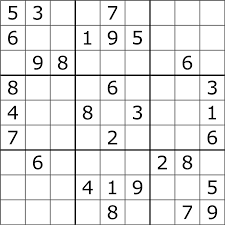
\includegraphics{sudoku}
\end{figure}

\newpage
\tableofcontents

% ==================================================================================

\newpage
\section{Introduction}

For a standard Sudoku, we have 9 rows and 9 columns. We have 9 possible digits in each square. So lets
define them as sets.  For other sized grids, the sets will change.  For the moment lets go with a 9x9 board.

% ==================================================================================

\section{Sets}

\begin{equation}
Digits=\lbrace1,2,3,4,5,6,7,8,9 \rbrace
\end{equation}

\begin{equation}
Rows=\lbrace1,2,3,4,5,6,7,8,9 \rbrace
\end{equation}

\begin{equation}
Columns=\lbrace1,2,3,4,5,6,7,8,9 \rbrace
\end{equation}

We will need some variables. For each cell we will have 9 variables, each a boolean. If the digit 8 is in the cell
the variable corresponding to 8 will be true, and all the others will be false.  So we will have a set of boolean values 
where 0 is false and 1 is true

We can add in a set of all possible cells

\begin{equation}
\begin{split}
Board = \lbrace (r,c) \rbrace  \\
\forall r\in Rows \\
\forall c \in Columns
\end{split}
\end{equation}

We need a set of booleans where we can use them for choices. 

\begin{equation}
Boolean=\lbrace 0,1 \rbrace
\end{equation}

% ==================================================================================

\section{Variables}

We will then have the following variables where the C conveys the concept of the choice in that cell. 

\begin{equation}
\begin{split}
C_{rcv} \\
\forall r \in Rows \\
\forall c \in Columns \\
\forall v \in Digits \\
where C_{rcv} \in Boolean
\end{split}
\end{equation}

To make writing some constraints simpler add in some new variables for the values in a given cell. Since this is a derived value it can be any number. 
In practice since it will be the sum of integers, it will be an integer.

\begin{equation}
\begin{split}
V_{rc} \\
\forall r \in Rows \\
\forall c \in Columns \\
V_{rc} \in Digits
\end{split}
\end{equation}

% ==================================================================================

\section{Constraints}

% ==================================================================================

\subsection{Basic Constraints}

To restrict the choices to just one in each cell, we need the following constraint.

\begin{equation}
\sum_{v \in Values} C_{rcv} = 1 , \forall r \in Rows, \forall c \in Columns
\end{equation}

For the constraint on the value variables, we add the following.

\begin{equation}
\sum_{v \in Values} v. C_{rcv} = V_{rc} ,  \forall r\in Rows, \forall c \in Columns
\end{equation}

% ==================================================================================

\subsection{Uniqueness}

Typically there are regions that impose a uniqueness condition. These work in a very similar way. If we have a set of the cells in the region

\begin{equation}
Region=\lbrace (r, c) \rbrace,  \forall (r, c) \in Region
\end{equation}

The we can impose the condition for uniqueness as follows.  Not all regions will have a full set of digits, so the \( \leq 1 \) condition needs to be applied. 
If the region has 9 cells, then all the sums will be 1. 

\begin{equation}
\sum_{ (r,c) \in Region} C_{rcv} \leq 1 , \forall v\in Digits
\end{equation}

% ==================================================================================

\subsection{Rows}

Rows now form 9 regions.

\begin{equation}
Row(i) = \lbrace  (i, c) s \rbrace , \forall c \in Column
\end{equation}

% ==================================================================================

\subsection{Columns}

Columns do the same

\begin{equation}
Column(i) = \lbrace  (r, i)  \rbrace , \forall r \in Rows
\end{equation}

% ==================================================================================

\subsection{Boxes}

In addition to the uniqueness restrictions on rows and columns, some puzzles have boxes that are 3x3. In a 9x9 sudoku there are 9 of them and we can number them
Boxes are numbered left to right, top to bottom. 

\begin{equation}
Boxes=\lbrace1,2,3,4,5,6,7,8,9 \rbrace
\end{equation}


So first we need to go from the box number to the centre cell of each box. 

\begin{equation}
Centre(i) =  ( (i-1)\: div\:3 + 2, (i-1)\: mod\:3 + 2) ,  \forall (r,c) \in Region
\end{equation}

We can now generate the Region of all centre cells of boxes

\begin{equation}
Centers(i) = \lbrace Centre(i)  \rbrace , \forall i \in Regions
\end{equation}

We can also generate the Regions for each box. First we create a set of offsets

\begin{equation}
Offsets = \lbrace -1,0,1 \rbrace
\end{equation}

Then

\begin{equation}
Boxes(i) = \lbrace Centre(i) + (x, y) , x \in Offsets, y \in Offsets \rbrace, \forall i \in Regions
\end{equation}

% ==================================================================================

\subsection{Diagonals}

We need two regions. One for the top left to bottom right diagonal, and one for the bottom left to top right. 

\begin{equation}
TLBR = \lbrace (x, x), \forall x \in Rows \rbrace
\end{equation}

\begin{equation}
\sum C_{rcv} = 1, \forall (r,c) \in TLBR
\end{equation}

\begin{equation}
BLTR = \lbrace (x, 10-x), \forall x \in Rows \rbrace
\end{equation}

\begin{equation}
\sum C_{rcv} = 1, \forall (r,c) \in BLTR
\end{equation}


% ==================================================================================

This sets up the abstract model for standard Sudokus. 

% ==================================================================================

\subsection{Known Values}

What we need to do now is make the model concrete by add in known digits.

They are easy to constrain. If the required digit in a cell (r,c)  is D, we can impose this condition.

\begin{equation}
V_{rc} = D
\end{equation}

So far that enables the solution of standard Sudokus. 

% ==================================================================================

\section{Sudoku Variants}

There are lots of Sudoku variants. Here are some of the variants and how to add constraints that enable them to be solved. 

\subsection{Odd Even}

Some puzzles restrict the choices that can be placed in cells to subsets of the digits.  For eaxample that they must be even or odd. So we can define those sets.

\begin{equation}
Odds=\lbrace1,3,5,7,9 \rbrace
\end{equation}

\begin{equation}
Evens=\lbrace2,4,6,8 \rbrace
\end{equation}

Then for a given cell (r,c) that has to be even or odd we can add one of the following constraints. Not that it is \( \notin \) as the set condition.  This is to force the choice
of that cell to have an odd value in the case of an even cell is not allowed, and vice versa for even digits in odd cells.

\begin{equation}
C_{rcv} = 0, \forall v \notin Evens
\end{equation}

\begin{equation}
C_{rcv} = 0, \forall v \notin Odds
\end{equation}

% ==================================================================================

\section{Lines}

There are sudoku puzzles based on lines where the elements on the lines are subject to restrictions.  Lines are represented as an ordered list

\begin{equation}
line = [(r,c)] \forall (r,c) \in Line
\end{equation}

\begin{equation}
n = length(line)
\end{equation}

% ==================================================================================

\subsection{German and Dutch Whispers}

A German Whisper line is a line in the puzzle. Adjacent digits on the line must have a difference of at least 5. 
That precludes a 5 appearing on the line since the adjacent number would have to be a 0 or a 10, and neither are valid numbers.
We can then add a constraint that disallows any 5 on the line. This condition is not strictly necessary, but it does cut down choices.

\begin{equation}
C_{r,c,5} = 0, \forall (r,c) \in Line
\end{equation}

For the interior cells on a German Whisper line, then 4 and 6 should be excluded if the cells are in a region that 
imposes uniqueness.  That is more difficult to implement since it involves working out if the three cells are in the same region or regions. 
So it is probably not worth implementing

A Dutch Whisper line is the same as a German Whisper line, except the difference has to be at least 4.

So if there are n cells on the line and the required difference is D, we can add these constraints

\begin{equation}
abs (V_{line[i]} - V_{line[i+1]} \geq D, \forall i \in \lbrace 1 ... n-1 \rbrace
\end{equation}

If the line forms a loop, then add an extra condition

\begin{equation}
abs (V_{line[1]} - V_{line[n]}) \geq D
\end{equation}

% ==================================================================================

\subsection{Arrows}

Arrow restrictions have a head of the line which is the sum of the other cells on the line. When the length of the line is n, for a simple one cell total we have.

\begin{equation}
V_{line[1]}^{m} = \sum_{i=2}^n V_{line[i]}
\end{equation}

For an arrow with multiple cells that make the head, we have the list of cells, and a count of the number of cells in the head. If the number of cells in the head is m, and we have n cells in total, including the head on the arrow, we have
this restriction. We can create the totals by adding up the hundreds digit, tens digit and unit digit. 

\begin{equation}
\sum_{i=1}^m 10^{m-i} V_{line[i]} = \sum_{i=m+1}^n V_{line[i]}
\end{equation}

The simple variant can be implemented by using the the more generic and setting m = 1.

% ==================================================================================

\subsection{Thermometer}

Thermometer come in two flavours. The first is a strict thermometer where the values must increase along the line. 

\begin{equation}
V_{line[i]} < V_{line[i+1]}, \forall i \in \lbrace 1 ... n-1 \rbrace
\end{equation}

% ==================================================================================

\subsection{FrozenThermometer}

The second is such that they do not need to increase, but must obey any uniqueness condition for the cells region.For the non-strict case we have

\begin{equation}
V_{line[i]} \leq V_{line[i+1]}, \forall i \in \lbrace 1 ... n-1 \rbrace
\end{equation}

% ==================================================================================

\subsection{Palindromes}


Palindromes are lines where the cell on the line matches the corresponding cell from the other end so digits read the same no mater wich way you read it. 

\begin{equation}
V_{line[i]} = V_{line[n-i]} , \forall i \in \lbrace 1 ...  \lfloor n /2 \rfloor \rbrace
\end{equation}

This works for circular palindrome lines. 

Query. Do all circular palindromes have to have an even number of cells? 

% ==================================================================================

\subsection{Renban}

A renban puzzle consists of a line. Numbers on the line must form a sequence of integers with no gaps. The numbers can appear in any order.
The constraints are to find the lowest number on the line, the highest or upper number on the line. The difference between the upper and lower bounds
must be the line length less one. 

\begin{equation}
lower \leq V_{line[i]}, \forall i
\end{equation}

\begin{equation}
upper \leq V_{line[i]}, \forall i
\end{equation}

Upper is always greater than lower, or equal if there is just one cell on the line which doesn't happen.  We can then take differences and we will always have a postive difference. 

\begin{equation}
upper - lower = n - 1
\end{equation}

Lastly, the values on the line must be unique

\begin{equation}
\sum_{d \in Digits} C_{d,line[i]} = 1, \forall i 
\end{equation}


% ==================================================================================

\subsection{Between the Ends}

A between the ends line has two ends with numbers in them.  The digits on the line must be between the two numbers. There are no uniqueness constraints other than the constraints imposed
by other rules.  The problem that needs to be solved is to get a lower value of the circles and the upper value of the circles. You don't know a priori which is the higher. Then the constaint for the 
numbers is easy.  It's also clear to work out that ones and nines cannot be on the line. 

\begin{equation}
V_{line[i]} < U, \forall i \notin \lbrace 1, n \rbrace
\end{equation}

\begin{equation}
V_{line[i]} > L, \forall i \notin \lbrace 1, n \rbrace
\end{equation}

% ==================================================================================

\subsection{Diagonal}

In a diagonal sudoku, either one or two diagonal lines are added. Along each diagonal, digits must be unique. 



% ==================================================================================

\subsection{Argyle}


% ==================================================================================

\section{Magic Squares}


Magic Squares are a 3 by 3 set of squares where the sum of any row, column or diagonal are the same. The total must be 15. Another
fact is that the centre square must be 5. 

The cells are labelled in the same way as boxes are numbered. A function returns the ordered list of the cells in the magic square.


\begin{equation}
magic(r,c) = [ (r+x, r+y), \forall y \in Offsets, \forall x \in Offsets ]
\end{equation}

A magic square is specified by its centre, (r,c).  The centre of a magic square must be 5. 

\begin{equation}
V_{magic[5]} = 5
\end{equation}

It's not necessary, but corners of magic squares must be even, and edges must be odd. 


\begin{equation}
C_{magic[i] v} = 0, \forall v \in Evens, \forall i \in \lbrace 1,3,7,9 \rbrace
\end{equation}

 and 

\begin{equation}
C_{magic[i] v} = 0, \forall v \in Odds, \forall i \in \lbrace 2,4,6,8 \rbrace
\end{equation}

The constraint sums are now implemented.

\begin{gather}
\sum_{i \in \lbrace 1,2,3 \rbrace} V_{magic[i]} = 15 \\
\sum_{i \in \lbrace 4,5,6 \rbrace} V_{magic[i]} = 15 \\
\sum_{i \in \lbrace 7,8,9 \rbrace} V_{magic[i]} = 15 \\
\sum_{i \in \lbrace 1,4,7 \rbrace} V_{magic[i]} = 15 \\
\sum_{i \in \lbrace 2,5,8 \rbrace} V_{magic[i]} = 15 \\
\sum_{i \in \lbrace 3,6,9 \rbrace} V_{magic[i]} = 15 \\
\sum_{i \in \lbrace 1,5,9 \rbrace} V_{magic[i]} = 15 \\
\sum_{i \in \lbrace 3,5,7 \rbrace} V_{magic[i]} = 15 
\end{gather}

% ==================================================================================

\section{Pairs}

Some of the variants look at the restriction between two different cells. 

For some of these we need a complete set of pairs on the board.


\begin{equation}
starts = Rows - \lbrace 9 \rbrace
\end{equation}

\begin{equation}
RowPairs = \lbrace  Pair ((r,c), (r+1, c), \forall r \in starts, \forall c \in starts \rbrace
\end{equation}

\begin{equation}
ColumnPairs = \lbrace  Pair ((r,c), (r, c+1), \forall r \in starts, \forall c \in starts \rbrace
\end{equation}

\begin{equation}
Pairs = RowPairs \cup ColumnPairs
\end{equation}

% ==================================================================================

\subsection {XV Sudoku}

TODO Image of XV Sudoku

XV Sudoku consists of a pair of orthogonally adjacent cells. If a Roman V is between the cells they add up to 5.
If an X is between the cells they total 10.  There are only two ways to make a 5, 1 and 4, 2 and 3. So we can add a new set to give the solver a helping hand.
For the two cells they can be defined as a line with two elements

\begin{equation}
vset=\lbrace 1,2,3,4 \rbrace
\end{equation}


\begin{equation}
C_{rcv} = 0, \forall v \notin vset, \forall (r,c) \in Pair
\end{equation}

Then we need the total for the V variant

\begin{equation}
\sum_{(r,c) \in Pair} V_{rc} = 5
\end{equation}

or for the X variant

\begin{equation}
\sum_{(r,c) \in Pair} V_{rc} = 10
\end{equation}

In some cases XV sudoku puzzles include the rule that all XV cells are given. In which case you are not allowed any non marked cells that sum to 5 or 10. 
This involves a \( \neq \) test, and that needs an addition boolean variable for each pair. 

TODO implement !=

% ==================================================================================

\subsection{Greater Than Sudoku}

Some puzzles contain greater than signs between two cells. The first of the pair must be less than the second of the pair. 

\begin{equation}
V_{pair[1]} < V_{pair[2]}
\end{equation}

This is a subset of Thermo Sudoku

% ==================================================================================

\subsection{Consecutive}

Typical represented by a white dot on the border between two cells. The requirement is that the two cells are consequtive. So if one of the cells is a 4
the other cell can only be a 3 or 5. 

The constraint is easy.

\begin{equation}
abs (V_{pair[1]} - V_{pair[2]}) = 1
\end{equation}

This is a subset of Renban Sudoki

% ==================================================================================

\subsection{Kropki}

Here it is typical that a white dot is placed on the border. The requirement is that the one of the values of the pair is twice the value of the other. 
That means that 5, 7 and 9 can never appear as digits on a Kropki pair.  There are only 8 possible combinations.

\begin{table}[h!]
\centering
\begin{tabular}{|c c|}
 \hline
 Pair[1] & Pair[2] \\
\hline
1 & 2 \\
2 & 1 \\
2 & 4 \\
3 & 6 \\
4 & 2 \\
4 & 8 \\
6 & 3 \\
8 & 4 \\
 \hline
\end{tabular}
\end{table}

We can eliminate 5, 7 and 9.

\begin{equation}
Kropki = \lbrace 1,2,3,4,6,8 \rbrace
\end{equation}

\begin{equation}
C_{rcv} = 0, \forall v \notin Kropki, \forall (r,c) \in Pair
\end{equation}

For the exact answer, introduce 8 binary variables corresponding to each of the possible combinations \( k_b \)

\begin{equation}
kropkis = \lbrace 12,21,24,36,42,48,63,84 \rbrace
\end{equation} 

Constrain the set to be unique, or use a SOS variabl
\begin{equation}
\sum_{b \in  kropkis} k_b = 1
\end{equation} 

\begin{equation}
b . k_{b} = 10.V_{r_1c_1} + V_{r_2c_2}
\end{equation} 

% ==================================================================================

\section{Chess Move}

There are a selection of restrictions based of chess moves. The typical implementation is to have a set of possible offsets from a cell. The
target cells are then generated from they (r,c) of the cell, and check to see if they are on the board. 

% ==================================================================================

\subsection{Fortress Sudoku}

In a fortress sudoku the cell that is the fortress is larger than the up to 4 orthogonally connected cells. If the fortress is (r,c) then

\begin{equation}
orthogonaloffsets = \lbrace  (-1,0), (0,-1), (0, 1),  (1,0), (1,1) \rbrace
\end{equation}

\begin{equation}
\begin{split}
V_{rc} > V_{r+x,c+y} \\ 
\forall (x,y) \in orthogonaloffsets, \\ 
 if (r+x, c+y) \in Board
\end{split}
\end{equation}

This a variant of Thermo Sudoku

% ==================================================================================

\subsection{Anti-king}

In an anti-king puzzle, no number may repeat a king's move away from another identical number.

TODO Diagram

The orthogonal move will not be possible because of the row and column restrictions, but if included
a good preprocessor will remove them.

\begin{equation}
\begin{split}
kingoffsets = \lbrace (-1,-1), (-1,0), (-1, 1), (0,-1), \\
 (0, 1), (1,-1), (1,0), (1,1) \rbrace
\end{split}
\end{equation}

For the restrictions we use the choice variables

\begin{equation}
\begin{split}
\sum_{v \in Values}  C_{rcv} = 0, \\
\forall (x,y) \in kingoffsets, \\
\forall (r,c) \in Board \\
if (r+x, c+y) \in Board
\end{split}
\end{equation}

% ==================================================================================

\subsection{Anti-knight}

For an anti knight move restriction is is the same as the anti-king except the offsets are different.

To do Diagram

\begin{equation}
\begin{split}
knightoffsets = \lbrace (-2,1), (-1,2), (1, 2), (2,1), \\
(-2,-1), (-1,-2), (1,- 2), (2,-1) \rbrace
\end{split}
\end{equation}

For the restrictions we use the choice variables

\begin{equation}
\begin{split}
\sum_{v \in Values}  C_{rcv} = 0, \\
\forall (x,y) \in knightoffsets,\\
\forall (r,c) \in Board \\
if (r+x, c+y) \in Board
\end{split}
\end{equation}

% ==================================================================================

\subsection{Donkey Step}

The same digit cannot appear in a cell within 2 diagonal steps from itself.

\begin{equation}
donkey_offsets = \lbrace  (-2,-2), (2,-2), (2, 2),  (-2,2), (1,1) \rbrace
\end{equation}

\begin{equation}
\begin{split}
abs (V_{rc} - V_{r+x,c+y}) \geq 2, \\ 
\forall (x,y) \in donkey_offsets, \\ 
\forall (r,c) \in Board \\
 if (r+x, c+y) \in Board
\end{split}
\end{equation}

% ==================================================================================

\subsection{Monkey Step}

The same digit cannot appear in a cell within 2 diagonal steps from itself.

\begin{equation}
monkey_offsets = \lbrace (-3,1), (-1,3), (1, 3), (3,1), \\
(-3,-1), (-1,-3), (1,- 3), (3,-1) \rbrace
\end{equation}

\begin{equation}
\begin{split}
abs (V_{rc} - V_{r+x,c+y}) \geq 2, \\ 
\forall (x,y) \in monkey_offsets, \\ 
\forall (r,c) \in Board \\
 if (r+x, c+y) \in Board
\end{split}
\end{equation}


% ==================================================================================

\subsection{Orthogonally Non Consecutive}

For orthogonally non consecutive rules, we need to make sure that if a 3 is in cell that any orthogonally adjacent cells are not 2 or 4.
That means the absolute difference between the two cells must be greater than or equal to two. We start off with the offsets, then implement the rules.

TODO Diagram

\begin{equation}
orthogonaloffsets = \lbrace  (-1,0), (0,-1), (0, 1),  (1,0), (1,1) \rbrace
\end{equation}

\begin{equation}
\begin{split}
abs (V_{rc} - V_{r+x,c+y}) \geq 2, \\ 
\forall (x,y) \in orthogonaloffsets, \\ 
\forall (r,c) \in Board \\
 if (r+x, c+y) \in Board
\end{split}
\end{equation}

An alternative implementation is to consider that there are effectively four Renban lines of length two. 

% ==================================================================================

\section{Regional Sum}

% ==================================================================================

\subsection{Killer}

In a killer sudoku, a region has a total denoted by S. The sum of the cells values in that region must be the same as the total.  Typically numbers cannot repeat
inside that region.  Note that a number does not have to appear in the region

TODO Diagram

\begin{equation}
region = \lbrace  (r,c)  | (r,c) \in Region \rbrace
\end{equation}

Then the total is easy. 

\begin{equation}
\sum_{(r,c) \in region} V_{rc} = S
\end{equation}

Uniqueness again is simple. 

\begin{equation}
\sum_{(r,c) \in region} C_{rcv} \leq 1, \forall v\in Digits
\end{equation}

% ==================================================================================

\subsection{Little Killer}

TODO Diagram

In a little killer sudoku, the same applies. The region is defined by a diagonal line labelled on the side with the total. There is no explicit uniqueness restriction. Numbers can repeat but there are the restrictions for uniqueness in boxes. 
The implementation is the same as that for a killer sudoku. 

In a quadruple sudoku at a junction of cells, there will be up to four digits specified. For example if the digits 678 appear in a circle, there must be at least one 6, one 7 and one 8 in the surrounding four cells. Digits can repeat. 

The cells form a 4 cell region, R.  If the digits are D = {a,b,c, d} then we can add these constraints. 

\begin{equation}
\sum_{(r,c) \in R} V_{rcv} \geq 1, \forall v \in D
\end{equation}

% ==================================================================================


\begin{itemize}
\item Disjoint Groups
\item Clones
\item Sandwich
\item Skyscraper
\item Jigsaw
\item Alternating Parity along a line
\item Snakes
\item Water
\item Rossini 
\item Indexing
\item Pointing Evens	Clover CTC 2022-01-27
\item Liar
\item nadir	CrackingTheCryptic
\item BALANCING SUDOKU 
\item Slingshot	A number in an arrow cell shows how many cells away the digit from which the arrow originates appears.
\item Unique Sums	Each cage sums to a unique number
\item X-Factor		Clues outside the grid show the product of the first X digits reading up, where X is the first digit.
\item Taxicab			Digits cannot appear a taxicab distance away from themselves

\end{itemize}



Preprocessing removes the redundant conditions. For example the value variables.  Putting these in makes the model readable and easier to code. 

Preprocessing with book keeping. 


Implementation

Pyomo

Yaml choices

Examples

Performance

Preprocessing reductions

Unique solutions

Branching counts
  
Book keeping

% ==================================================================================


\section{Formulations}

\subsection{Abs}

To implement an absolute function, \( z=|f(x)| \) we need to reformulate into two expressions: \( z = x \: if \: x \geq 0\: and \: -z=x\: if \: x< 0 \)

\subsection{Not equal}

\subsection{In Set}

\subsection{Not In Set}


\begin{figure}[!hb]
\centering
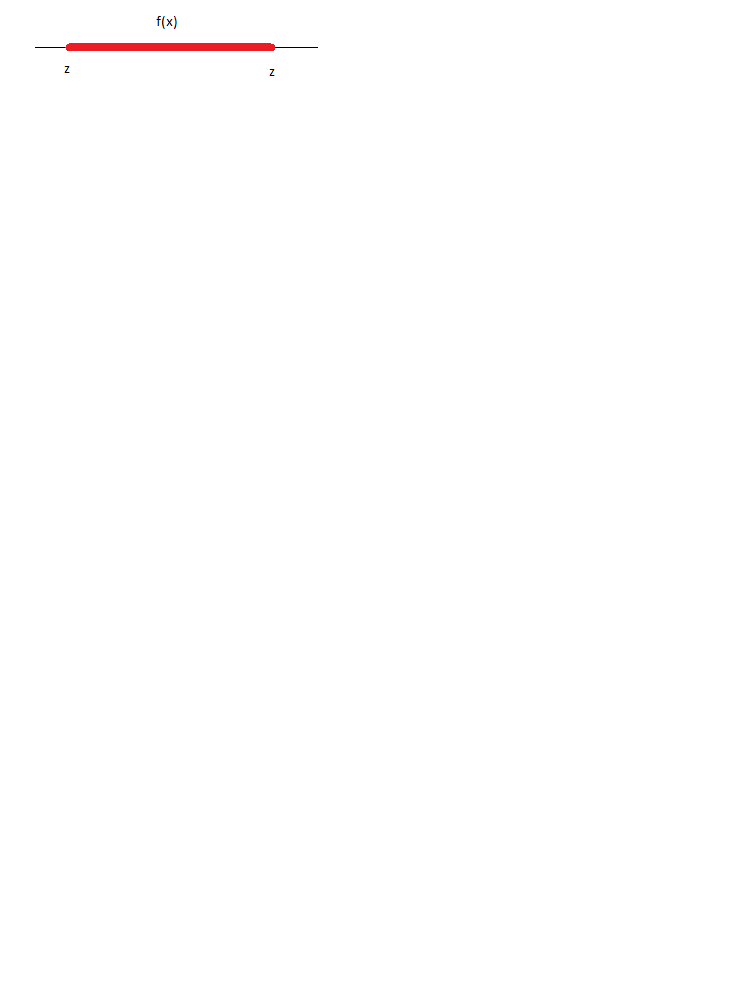
\includegraphics{numberline}
\end{figure}

Anti-Knight.  No digit may be a knght's move away from an identical digit.
Anti-King.  No digit mabe a king's move away from an identical digit.
Anti-Queen. No digit that follows the rule may be a queen's move away from an identical move. 
Thermometers. In a thermometer, the lowest digit is at the bulb end and strictly increases along its length. 
Non Consecutive. No digit can be orthoganally adjacent to a consecutive digit. 
Magic Square. In the marked 3x3 box, every row, column and diagonal must sum to the same number. 
Killer Sudoku: Cells are grouped into cages with dotted outlines.  The small number in the top left of each cage gives the sum of all digits inside it. Cages cannot contain repeated digits.

Square Quadruples. Each circled number gives between 1 and 4 digits that must be included in the surrounding four clls. Digits can repeat subject to other restrictions. 
Diagonals: The cells along a marked diagonal must contain the digits 1 to 9. 
Taxicab. The taxicab disatance between two cells is the minimum number of orthogonal moves needed to travel from one cell to the other. [Manhattan distance]
Kropki. A black dot between two cells means a digit on one side is double the digit on the other side. [Not all black dots are give] Complete or incomplete
Arrowheads. An arrowhead between two cells points at the lower digit.
Arrow Sum: The digit in the circle on an arrow is the sum of the other digits on the arrow.  [Unique?]
Multi digit Arrow Sum. 
Little Killer. Each clue with an arrow outside the grid shows the sum of the digits along the direction of the arrow. Digits can repeat subject to other restrictions
Jousting knights: Every digit must be a knights move away from at least one identical digit. 
Dominos: The sum of any two orthoganally adjacent digits can never be a number that is diviisble by 5. {5,10,15}
Killer Sudoku Hidden Sum. All cages sum to the same number that is to be determined. 
Palindromes. Market lines are palindromes. The digits along the line read the same in both dirctions. 
SumX. Orthoganally adjacent digits do not sum to 10 unless there is an X between them
SumV. Orthoganally adjacent digits do not sum to 5
N-Sums:
N-Products: 
Consequtive Lines:
Sandwich Sums
Odd Digits
Even Digits
Diagonal Pair Sums. Not all circles given CTC p111
Galactic Thermos. 
159 Sudoku
GAS 238 – Battenburg 
Normal sudoku rules apply. Every time a blue square appears at the intersection of four cells, the odd and even digits in those four cells must be in a 'checkerboard' pattern (two odd digits diagonally opposite each other, and two even digits diagonally opposite each other). Every time a white square appears at an intersection of four cells, the odd and even digits in those four cells must NOT be in a 'checkerboard' pattern. 
Frozen Thermometer


\end{document}